\documentclass[xetex,mathserif,serif]{beamer}
\usepackage{polyglossia}
\setdefaultlanguage[babelshorthands=true]{russian}
\usepackage{minted}
\usepackage{csquotes}

\useoutertheme{infolines}

\setmainfont{FreeSans}
\newfontfamily{\russianfonttt}{FreeSans}

\definecolor{links}{HTML}{2A1B81}
\hypersetup{colorlinks,linkcolor=,urlcolor=links}

\beamertemplatenavigationsymbolsempty

\title{ВКР}
\author[Юрий Литвинов]{Юрий Литвинов \newline \textcolor{gray}{\small\texttt{y.litvinov@spbu.ru}}}
\date{22.02.2025}

\begin{document}

    \frame{\titlepage}

    \section{Регламент}

    \begin{frame}
        \frametitle{Формальности}
        \begin{itemize}
            \item Курс \enquote{Преддипломная практика}:
            \begin{itemize}
                \item Отзыв научника на \textbf{преддипломную практику}
                \item Черновик текста ВКР
                \begin{itemize}
                    \item Титульник, на котором написано \enquote{Отчёт по преддипломной практике}
                \end{itemize}
                \item Непредпредзащита, то есть выступление на этой паре
            \end{itemize}
            \item Предзащита --- где-то за две недели до защиты, генеральная репетиция
            \item Защиты --- с 15 мая по 15 июня
            \item Начало июля --- выдача диплома
        \end{itemize}
    \end{frame}

    \begin{frame}
        \frametitle{Предварительные даты}
        \begin{itemize}
            \item Кафедра информатики, кафедра ПА --- 24 мая
            \item Кафедра ИАС --- 28 мая
            \item Кафедра СП, техпрог --- 7 и 9 июня
            \item ПИ --- 11 июня
        \end{itemize}
    \end{frame}

    \begin{frame}
        \frametitle{Документы для защиты}
        \begin{itemize}
            \item Сданная весенняя сессия
            \begin{itemize}
                \item С долгами (любыми) к защите не допускают
                \item Сессия в конце апреля
            \end{itemize}
            \item Текст диплома --- за две недели до защиты (строго, но включительно), в Blackboard
            \item Аннотация --- абзац текста, про что ВКР, в Blackboard (в т.ч. на английском)
            \item Отзыв научного руководителя --- за пять дней до защиты
            \item Отзыв рецензента --- за пять дней до защиты
            \begin{itemize}
                \item Они не так строго, потому что формально это не ваше дело
                \item Формально можно защищаться без отзыва и/или рецензии, но...
            \end{itemize}
            \item Научник должен быть на защите, рецензент не обязательно
        \end{itemize}
    \end{frame}

    \begin{frame}
        \frametitle{Кто такой ГЭК}
        \begin{itemize}
            \item ГЭК --- Государственная Экзаменационная Комиссия
            \item Формируется из ведущих специалистов в отрасли (не менее 50\%) и преподавателей СПбГУ
            \begin{itemize}
                \item У нас это обычно директора или начальники отделов уважаемых компаний
                \item Есть и молодые специалисты, понимающие в технологиях и не стесняющиеся задавать вопросы
            \end{itemize}
            \item Обычно 6-7 человек
            \item ГЭК формируется для направления, то есть бакалавры техпрога могут защищаться только в ГЭК для СВ.5162
        \end{itemize}
    \end{frame}

    \begin{frame}
        \frametitle{Как проходит защита}
        \framesubtitle{И как ставятся оценки}
        \begin{footnotesize}
            \begin{itemize}
                \item За одно заседание защищается максимум 8 человек, максимум 2 заседания в день (бывает \enquote{два с половиной})
                \item Порядок защиты фиксируется (когда вас распределяют по датам)
                \begin{itemize}
                    \item \footnotesize{Приказ о допуске к защите --- где-то в начале-середине мая}
                \end{itemize}
                \item Выступление защищающегося, вопросы от членов ГЭК и аудитории, отзыв научника, рецензия (зачитывается научником, если рецензента нет), вопросы по отзыву/рецензии, ответное слово (если надо)
                \item ГЭК совещается (по окончании заседания)
                \item Члены ГЭК выставляют оценки по критериям, каждый независимо
                \begin{itemize}
                    \item \footnotesize{См. \url{https://edu.spbu.ru/gia.html}}
                \end{itemize}
                \item Каждый член ГЭК ставит итоговую оценку (при этом критерии --- это только рекомендации), оценки всех членов ГЭК усредняются и ставится итоговая
                \begin{itemize}
                    \item \footnotesize{Оценки научника и рецензента непосредственно не учитываются! Они имеют рекомендательное значение для ГЭК.}
                \end{itemize}
                \item Итоговая оценка заносится в протокол защиты и выставляется на Blackboard
                \item Защищающихся приглашают, оглашают результаты, поздравляют с присвоением квалификации (или нет)
            \end{itemize}
        \end{footnotesize}
    \end{frame}

    \section{Отчёт}

    \begin{frame}
        \frametitle{Отчёт, структура}
        \begin{itemize}
            \item Титульный лист
            \item Оглавление
            \item Введение в предметную область, постановка задачи
            \item Обзор литературы и существующих решений
            \item Описание предлагаемого решения
            \begin{itemize}
                \item Отдельно архитектура и детали реализации
            \end{itemize}
            \item Апробация и/или эксперименты
            \item Заключение
            \item Список литературы
            \item Не более 40 страниц (60 для магистров)
            \item Требования к оформлению: \url{https://edu.spbu.ru/gia.html}
        \end{itemize}
    \end{frame}

    \begin{frame}
        \frametitle{Введение}
        \begin{columns}
            \begin{column}{0.6\textwidth}
                \begin{itemize}
                    \item Известная информация, \enquote{Background}
                    \item Неизвестная информация, \enquote{Gap}
                    \begin{itemize}
                        \item Актуальность темы
                        \item Практическая значимость
                        \item Кому конкретно это надо
                    \end{itemize}
                    \item Кратко про ваш подход к решению задачи, почему он приведёт к успеху (\enquote{Гипотеза} и \enquote{Подход})
                    \item Этот раздел заслуживает особого внимания!
                \end{itemize}
            \end{column}
            \begin{column}{0.4\textwidth}
                \begin{center}
                    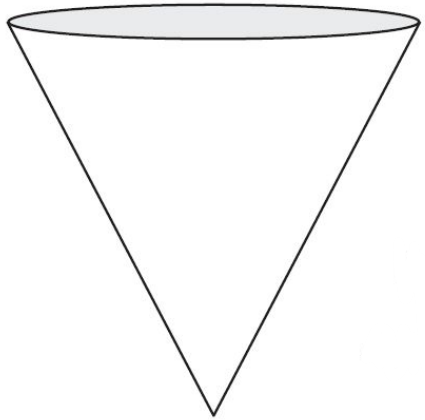
\includegraphics[width=\textwidth]{introductionCone.png}
                \end{center}
            \end{column}
        \end{columns}
    \end{frame}

    \begin{frame}
        \frametitle{Постановка задачи}
        \begin{itemize}
            \item Цель работы
            \begin{itemize}
                \item Одним предложением --- что конкретно надо сделать
            \end{itemize}
            \item Задачи
            \begin{itemize}
                \item Отчуждаемые
                \item Специфичные
                \item Решение которых приведёт к цели
                \item Выполнить обзор, спроектировать, реализовать, выполнить апробацию/эксперименты
            \end{itemize}
        \end{itemize}
    \end{frame}

    \begin{frame}
        \frametitle{Обзор}
        \begin{itemize}
            \item Обзор существующих решений
            \begin{itemize}
                \item Цель обзора, критерии отбора материалов
                \item Критерии сравнения
                \item Таблица с результатами
                \item Выводы
            \end{itemize}
            \item Обзор используемых чужих результатов
            \begin{itemize}
                \item Всё, написанное и придуманное не вами --- в обзор
            \end{itemize}
            \item Должен соотноситься с темой и целью
        \end{itemize}
    \end{frame}

    \begin{frame}
        \frametitle{Описание решения}
        \begin{itemize}
            \item Разделы должны соответствовать списку задач
            \item Аргументированное обоснование принятых решений и отказа от альтернатив
            \item Выбор инструментария
            \item Описание архитектуры, алгоритмов и т.п.
            \item Описание того, над чем \enquote{пришлось подумать больше пяти минут}
        \end{itemize}
    \end{frame}

    \begin{frame}
        \frametitle{Описание решения (2)}
        \begin{itemize}
            \item Рисунки и диаграммы
            \begin{itemize}
                \item Лучше использовать стандартную нотацию (UML, ER, ...)
                \item Подписи, единицы измерения
                \begin{itemize}
                    \item Чужие рисунки --- со ссылкой на источник
                \end{itemize}
                \item Ссылки из текста
                \item Сквозная нумерация
            \end{itemize}
            \item Таблицы
            \begin{itemize}
                \item Единицы измерения в заголовке
                \item Чтобы было всё видно даже в напечатанном варианте
            \end{itemize}
        \end{itemize}
    \end{frame}

    \begin{frame}
        \frametitle{Апробация/эксперименты}
        \begin{itemize}
            \item В любом случае должна быть
            \begin{itemize}
                \item Для чисто инженерных работ --- апробация на реальных пользователях
            \end{itemize}
            \item Лучше численный результат, ещё лучше --- если его можно с кем-то сравнивать
            \begin{itemize}
                \item System Usability Scale
            \end{itemize}
            \item \textbf{Матстат}
            \item Никаких лишних цифр после запятой
            \item Эксперимент должен быть согласован с постановкой задачи
            \item Threats to validity
            \item Выводы
        \end{itemize}
    \end{frame}

    \begin{frame}
        \frametitle{Заключение}
        \begin{itemize}
            \item Перечисление результатов, выносимых на защиту
            \item Должно быть согласовано с постановкой задачи (вплоть до полного её повторения, но с уточнением по полученным результатам)
            \item Должно быть согласовано с текстом
            \begin{itemize}
                \item Никаких результатов из ниоткуда
            \end{itemize}
            \item Ссылка на репозиторий или пара слов про то, почему её нет и что вы можете показать взамен
            \begin{itemize}
                \item ...Было внедрено, отзыв о внедрении прилагается
            \end{itemize}
            \item Благодарности (прежде всего консультанту)
            \item Может быть, Future work
            \item Этот раздел также заслуживает особого внимания!
        \end{itemize}
    \end{frame}

    \begin{frame}
        \frametitle{Литература}
        \begin{itemize}
            \item Cсылок примерно как страниц в работе
            \item Обязательно на каждый пункт ссылаться из текста
            \item Лучше ссылаться на научные статьи
            \begin{itemize}
                \item Ещё лучше --- на книги, но по предметной области
                \item Смотрите на индекс Хирша и число цитирований
            \end{itemize}
            \item Реально прочитанные работы
        \end{itemize}
    \end{frame}

    \begin{frame}
        \frametitle{Литература (2)}
        \begin{itemize}
            \item ГОСТ Р 7.0.5-2008
            \begin{itemize}
                \item А.Н. Терехов, Т.А. Брыксин, Ю.В. Литвинов и др., Архитектура среды визуального моделирования QReal. // Системное программирование. Вып. 4. СПб.: Изд-во СПбГУ. 2009, С. 171-196
                \item Порядок --- алфавитный (по авторам), в порядке упоминания в тексте, в хронологическом порядке (если это важно)
                \item Ссылки в тексте --- номер в квадратных скобках: \enquote{блаблабла [1]} (с пробелом)
            \end{itemize}
            \item В литературу --- только, гм, литературу
            \begin{itemize}
                \item Подстраничные сноски для ссылок на сайты, статьи на Хабре и т.д.
                \item Электронные источники в списке литературы допустимы (надо указывать дату обращения)
            \end{itemize}
        \end{itemize}
    \end{frame}

    \section{Презентация}

    \begin{frame}
        \frametitle{Презентация, структура}
        \begin{itemize}
            \item Титульный слайд
            \item Введение (примерно 1-2 слайда)
            \item Постановка задачи (1 слайд)
            \item Обзор (примерно 1 слайд)
            \item Предлагаемое решение (примерно 1 слайд)
            \item Апробация/эксперименты (примерно 1 слайд)
            \item Результаты, выносимые на защиту (1 слайд) --- обязательно, последним слайдом
        \end{itemize}
    \end{frame}

    \begin{frame}
        \frametitle{Демо}
        \begin{itemize}
            \item Короткий видеоролик/gif, на 1-2 минуты сверх выделенных на выступление
            \item Не обязательно, но ГЭК очень любит
            \item Даже если это библиотека/консольное приложение, тоже ок, покажите консоль
            \begin{itemize}
                \item Только чтобы всё было видно
            \end{itemize}
            \item Если работа закрытая, даже демонстрировать может быть нельзя, согласуйте с начальством
        \end{itemize}
    \end{frame}

    \begin{frame}
        \frametitle{Тактические соображения}
        \begin{itemize}
            \item Укладывайтесь в 7 минут
            \item Стоит порепетировать самим и перед научником
            \item По протоколу положены вопросы
            \begin{itemize}
                \item Если не хотите неожиданных, можно намеренно оставить некую недосказанность
                \item И подготовить скрытые слайды
                \item Тем не менее, неожиданные вопросы будут!
            \end{itemize}
            \item Не увлекайтесь техническими подробностями
            \item Не увлекайтесь их отсутствием
            \item Избегайте больших формул на слайдах
            \item Слайды должны быть такими, чтобы вас можно было особо не слушать
            \begin{itemize}
                \item Расшифровка сокращений, визуализация всего, название-авторы статей и т.п.
            \end{itemize}
        \end{itemize}
    \end{frame}

    \section{Общие рекомендации}

    \begin{frame}
        \frametitle{Общие рекомендации}
        \begin{itemize}
            \item Никакого заимствования 
            \begin{itemize}
                \item Сдача чужой работы --- отчисление без права восстановления сразу
                \item Копипаст даже одного предложения без указания источника --- незачёт
                \item Правильно оформленный копипаст --- нехорошо
            \end{itemize}
            \item Обязательно показать и текст, и презентацию научнику перед отсылкой рецензенту
            \begin{itemize}
                \item Порепетировать выступление!
            \end{itemize}
        \end{itemize}
    \end{frame}

    \begin{frame}
        \frametitle{Оформление кода}
        \begin{itemize}
            \item Рецензент может (и должен!) смотреть на код
            \item Аккуратные исходники со стайлгайдом и комментариями
            \item README 
            \begin{itemize}
                \item Общее описание проекта
                \item Описание процесса сборки
                \item Описание воспроизведения эксперимента
                \item У рецензента должно получиться то же, что и у вас, без вашей помощи
            \end{itemize}
            \item Настроенный и проходящий билд в CI-системе
            \item Лицензия (какая хотите, мы рекомендуем Apache License 2.0 или MIT)
            \item Желательно, всё по-английски
        \end{itemize}
    \end{frame}

    \begin{frame}
        \frametitle{Полезные ресурсы}
        \begin{itemize}
            \item Сайт кафедры --- \url{https://se.math.spbu.ru/}
            \begin{itemize}
                \item Раздел \enquote{Студентам} --- архив работ
            \end{itemize}
            \item Титульники --- \url{https://github.com/spbu-se/matmex-diploma-template}
            \item Презентация --- \url{https://github.com/spbu-se/report_presentation_template}
            \item Онлайн-редакторы TeX --- \url{https://papeeria.com/}, \url{https://www.overleaf.com/}
            \item Чеклист по презентациям --- \url{https://goo.gl/UeDRff}
        \end{itemize}
    \end{frame}

    \begin{frame}
        \frametitle{FAQ}
        \begin{itemize}
            \item Можно ли поменять научника/тему диплома?
            \begin{itemize}
                \item Да, где-то до 25-го апреля
                \item По заявлению в учебный отдел за подписью старого и нового научника 
                \item Форма заявления: \url{https://disk.yandex.ru/i/r-gPcPixqrPYRQ}
            \end{itemize}
            \item Можно ли поменять рецензента?
            \begin{itemize}
                \item Формально рецензента вам назначают, так что студент инициировать смену рецензента не может
                \item Неформально, написать мне, и \textit{возможно}, УОП поправит приказ
            \end{itemize}
            \item Можно ли перенести защиту?
            \begin{itemize}
                \item Нет. Либо вы защищаетесь, либо отчисляетесь по незащите ВКР с правом восстановиться для защиты
                \item Теоретически можно закрыть справкой две недели до защиты (чтобы не получить неуд за невыкладывание текста) и две недели до резервного дня, тогда защиту перенесут на осень
                \item Академ --- тоже вариант, но только по уважительной причине
            \end{itemize}
        \end{itemize}
    \end{frame}

\end{document}